%========================
% Theme
%========================
\documentclass[8pt]{beamer}
\setbeamersize{text margin left=10mm,text margin right=10mm} 
\usetheme[progressbar=frametitle]{metropolis}
\usepackage{appendixnumberbeamer} % handles appendix slide numbering

%========================
% Packages: Icons and Tables
%========================
\usepackage{booktabs}        % professional tables
\usepackage[scale=1]{ccicons} % Creative Commons icons

%========================
% Packages: Plots and TikZ
%========================
\usepackage{pgfplots}
\usepgfplotslibrary{dateplot}

\usepackage{tikz}
\usetikzlibrary{positioning}

%========================
% Packages: Algorithms
%========================
\usepackage{algorithm}
\usepackage{algpseudocode}

%========================
% Packages: Math
%========================
\usepackage{amsmath,amsfonts,amsthm,amssymb}
\usepackage{mathtools}
\newtheorem{prop}{Proposition}

%========================
% Custom commands
%========================
\usepackage{xspace}
\newcommand{\themename}{\textbf{\textsc{metropolis}}\xspace}

%========================
% Custom footline
%========================
\setbeamertemplate{footline}
{%
  \leavevmode%
  \hbox{%
  \begin{beamercolorbox}[wd=.35\paperwidth,ht=2.5ex,dp=1.5ex,center]{author in head/foot}%
    \usebeamerfont{author in head/foot}\insertshortauthor
  \end{beamercolorbox}%
  \begin{beamercolorbox}[wd=.3\paperwidth,ht=2.5ex,dp=1ex,center]{title in head/foot}%
    \usebeamerfont{title in head/foot}\insertshorttitle
  \end{beamercolorbox}%
  \begin{beamercolorbox}[wd=.3\paperwidth,ht=2.5ex,dp=1ex,right]{date in head/foot}%
    \usebeamerfont{date in head/foot}\insertframenumber{} / \inserttotalframenumber
  \end{beamercolorbox}}%
  \vskip0pt%
}

%========================
% Remove default navigation symbols
%========================
\setbeamertemplate{navigation symbols}{}

\usepackage{pgf,pgfarrows,pgfnodes,pgfautomata,pgfheaps,pgfshade}
\usepackage{hyperref}
\usepackage{listings}
\usepackage{color}

\lstset{language=R,
    basicstyle=\small\ttfamily,
    stringstyle=\color{DarkGreen},
    otherkeywords={0,1,2,3,4,5,6,7,8,9},
    morekeywords={TRUE,FALSE},
    deletekeywords={data,frame,length,as,character},
    keywordstyle=\color{blue},
    commentstyle=\color{DarkGreen},
}

\usepackage{xcolor}

\lstset{
    language=Python,
    basicstyle=\ttfamily\small,
    keywordstyle=\color{blue},
    commentstyle=\color{gray},
    stringstyle=\color{red},
    breaklines=true,
    numbers=left,
    numberstyle=\tiny
}



%%%%%%%%%%%%%%%%%%%%%%%%%%%%%%%%%%%%%%%%%%%%%%%%%%%%%%%%%%%%%%%%%%%%
%%%%%%%%%%%%%%%%%%%%%%%%%%%%%%%%%%%%%%%%%%%%%%%%%%%%%%%%%%%%%%%%%%%%
% AQUI SE DEFINEN LAS IMAGENES PARA UTILIZAR DESPUES
%\pgfdeclareimage[interpolate=true, height=7cm,width=16cm]{halton-points}{halton-points}
%\pgfdeclareimage[interpolate=true, height=3cm, width =4cm]
%{serie-petroleo-reducido}{serie-petroleo-reducido}
%\pgfdeclareimage[interpolate=true, height=3cm, width =4cm]{rectangle-triangle}{rectangle-triangle}
%\pgfdeclareimage[interpolate=true, height=3cm, width =4cm]{any-angle}{any-angle}
%\pgfdeclareimage[interpolate=true, height=3cm, width =4cm]{Pythagoras}{Pythagoras}


\title{Chapter 1 - Random Number Generation}
\subtitle{Rejection Sampling}
\author{Prof. Alex Alvarez, Ali Raisolsadat}
\institute{School of Mathematical and Computational Sciences \\ University of Prince Edward Island}
\date{} % leave empty or add \today
%\title[Stat 4110]{Stat 4110 Statistical Simulation}
%\subtitle{}
%\author[University of Prince Edward Island]{School of Mathematical and Computational Sciences \\ University of Prince Edward Island}

%========================
% Begin document
%========================
\begin{document}

%-------------------
% Title frame
%-------------------
\maketitle

%-------------------
% Slide 1: Review: Inverse Transform Method
%-------------------
\begin{frame}{Review: Inverse Transform Method}
The following graph corresponds to a histogram of a sample of 2000 generated random numbers uniformly distributed in $[0,1]$.
Let's refer to this as the $U$ distribution.

\begin{center}
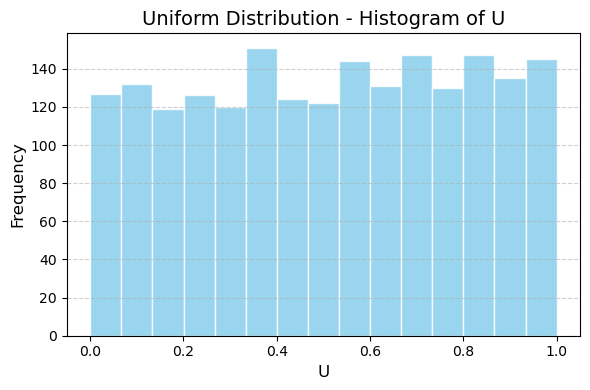
\includegraphics[width=\textwidth]{chapter1-part3-plot1.png}
\end{center}

\end{frame}


%-------------------
% Slide 2: Review: Inverse Transform Method - Histogram
%-------------------
\begin{frame}{Review: Inverse Transform Method}
The following graph corresponds to a histogram of a sample of 1000 generated random numbers distributed according to the p.d.f. given by $f(x)=2x$ in $[0,1]$ and 0 otherwise. The inverse transform method was used to generate the sample. Let's refer to this as the $X$ distribution.

\begin{center}
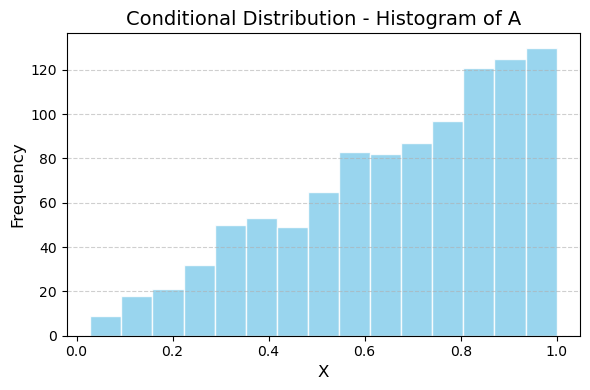
\includegraphics[width=\textwidth]{chapter1-part3-plot2.png}
\end{center}
\end{frame}

%-------------------
% Slide 3: Introduction to Rejection Sampling
%-------------------
\begin{frame}{Introduction to Rejection Sampling}
\textbf{Observation}:

\vspace{2mm}

At an intuitive level, it seems that we can get a sample similar to the one in the histogram of the X Distribution by discarding/rejecting some of the values in the sample taken from the U Distribution.  

\vspace{2mm}

If we were to do this in this example, it seems that we should reject more of the smaller individual values and less of the larger individual values from the $U$ sample.

\vspace{2mm}

This informal reasoning is the main idea behind the method known as \textbf{Rejection Sampling}. 
\end{frame}


%-------------------
% Slide 4: Introduction to Rejection Sampling
%-------------------
\begin{frame}{Introduction to Rejection Sampling}
\textbf{Rejection Sampling}

\vspace{2mm}

Suppose that our objective is to \textbf{generate a sequence of random numbers that follow a distribution with density $f$}. \textbf{Let's refer to $f$ as the target density}.

\vspace{2mm}

We will start with a sequence of random numbers from a distribution with density $g$ (the proposal density) which we know how to generate and we will \textbf{reject} some of these generated random numbers in order to achieve a new sequence of random numbers that follows the target distribution.
\end{frame}


%-------------------
% Slide 5: Introduction to Rejection Sampling
%-------------------
\begin{frame}{Introduction to Rejection Sampling}
\textbf{Questions}: 

\begin{itemize}
\item Is it always possible to achieve the target distribution in this way?
\item How do we decide which random numbers are accepted/rejected?
\end{itemize}

\pause

In order to achieve the target distribution we should start with a proposal distribution that can take the same values as the target distribution.
For example, if the target distribution is the exponential distribution, which takes values in the interval $(0,\infty)$, we cannot use the uniform distribution in $[0,1]$
as the proposal distribution, as we will never be able to get a proposal random number greater than 1.

\vspace{2mm}
\pause

The algorithm that follows answers the question of how to reject some of the proposal random numbers in order to achieve a sample that follows the target distribution. 
\end{frame}


%-------------------
% Slide 6: Rejection Sampling
%-------------------
\begin{frame}{Rejection Sampling}
\textbf{Basic Rejection Sampling Algorithm}

Consider a target density $f$ and a proposal density $g$ such that there exists a function $p$ taking values in $[0,1]$ such that 
\begin{equation*}
f(x)=\frac{1}{Z}p(x)g(x)  \; \text{ where } Z=\int p(x) g(x) dx
\end{equation*}

\alert{Algorithm}

To generate one random number from the target distribution:

\begin{enumerate}
	\item Generate $Y$ (the proposal) with density $g$ 
	\item Generate $U \sim U[0,1]$
	\item {\bf if} $U \leq p(Y)$ then \\
       $X=Y$ (meaning that $Y$ is accepted)\\  
	\item else return to Step 1
	\item Return $X$
\end{enumerate}
\end{frame}

%-------------------
% Slide 7: Rejection Sampling Proof
%-------------------
\begin{frame}{Rejection Sampling Proof}
\textbf{Proof}.
We have
\begin{align*}
P(X = x) &= \sum_{n=1}^{\infty} P(\text{reject $n-1$ times, draw $Y = x$ and accept it})\\
&= \sum_{n-=1}^{\infty}P(\text{reject $Y$})^{n-1}P(\text{draw $Y = x$ and accept it})
\end{align*}
Then
\begin{align*}
& P(\text{draw $Y = x$ and accept it})\\
&= P(\text{draw $Y = x$})P(\text{accept $Y|Y=x$})\\
&= g(x)P\biggl(U \leq p(y)| Y = x \biggl) \\
&= g(x)P\biggl(U \leq Z\frac{f(y)}{g(y)} \biggl| Y = x \biggl)\\
&= Zf(x)
\end{align*}
\end{frame}

%-------------------
% Slide 8: Rejection Sampling Proof
%-------------------
\begin{frame}{Rejection Sampling Proof}
The probability of having a rejection is 
\begin{align*}
P(\text{reject $Y$}) 
&= \sum_{x\in\Omega} P(\text{draw $Y = x$ and reject it}) \\
&= \sum_{x\in\Omega} g(x)P\biggl(U \geq Z\frac{f(y)}{g(y)} \biggl| Y = x \biggl)\\
&= \sum_{x\in\Omega} g(x) \biggl(1 - Z\frac{f(x)}{g(x)} \biggl) = 1- Z
\end{align*}
Hence we have 
\begin{align*}
P(X = x) 
&= \sum_{n=1}^{\infty} P(\text{reject $n-1$ times, draw $Y = x$ and accept it})\\
&= \sum_{n=1}^{\infty}(1-Z)^{n-1}Zf(x)\\
&= f(x)Z \sum_{n=1}^{\infty}(1-Z)^{n-1} \quad \biggl(\text{Note: $\sum_{n=1}^{\infty}r^{n-1} = \frac{1}{1-r}$ for $|r| < 1$}\biggl)\\
&= Zf(x)\frac{1}{1-(1-Z)} = f(x)
\end{align*}
\end{frame}

%-------------------
% Slide 9: Rejection Sampling
%-------------------
\begin{frame}{Rejection Sampling}
\textbf{Remarks}

\begin{itemize}
	\item The number of proposals used to generate one accepted value is random.
	\item Actually, the number of proposals used to generate one accepted value has geometric probability distribution with mean $1/Z$
	\item $Z$ also represents the probability that one proposal is accepted, so the higher the value of $Z$ the most efficient is the algorithm.
\end{itemize}
\end{frame}


%-------------------
% Slide 10: Rejection Sampling Example
%-------------------
\begin{frame}{Rejection Sampling Example}
The initial example in these slides correspond to the proposal density given by $g(x)=1$ in $[0,1]$, and target density $f(x)=2x$ also in $[0,1]$. Outside of this interval both densities are null.

\vspace{2mm} 

We also know that in order to apply the previous algorithm we need a function $p$ taking values in $[0,1]$ such that 
\begin{equation*}
f(x)=\frac{1}{Z}p(x)g(x)  \; \text{ where } Z=\int p(x) g(x) dx
\end{equation*}

After substituting $f$ and $g$ we get
\begin{equation*}
p(x)=Z\cdot2x
\end{equation*}

As $0\leq p(x) \leq 1$ for all $x \in [0,1]$ then $2Z \leq 1$ or $Z \leq 1/2$.

\vspace{2mm}

This means that any value $0<Z\leq 1/2$ is a valid choice for the algorithm, with $Z=1/2$ being the best choice.
\end{frame}


%-------------------
% Slide 11: Rejection Sampling Example
%-------------------
\begin{frame}[fragile]
\alert{Code}

\vspace{2mm}

\begin{columns}
\column{0.4\textwidth}
{\bf R Code:}
\begin{lstlisting}
counter <- 1
U <- vector();
A <- vector();
for (i in c(1:2000)){ 
  U[i] <- runif(1)
  D <- runif(1)
  if (D < U[i]){
    A[counter] = U[i];
    counter <- counter+1;
  }
}
accepted <- counter-1
hist(U)
hist(A)
\end{lstlisting}

\column{0.45\textwidth}
{\bf Python Code:}
\begin{lstlisting}
import numpy as np
import matplotlib.pyplot as plt

counter = 0
U = []
A = []

for i in range(2000):
    u = np.random.uniform()
    d = np.random.uniform()
    U.append(u)
    if d < u:
        A.append(u)
        counter += 1

plt.hist(U, bins=20)
plt.show()

\end{lstlisting}
\end{columns}
\end{frame}


%-------------------
% Slide 12: Envelope Rejection Sampling
%-------------------
\begin{frame}{Envelope rejection sampling}
The envelope rejection sampling algorithm can be used even in cases when we start with a non-normalized target density $f$ (meaning that $\int f(x) dx \neq 1$).

\vspace{2mm}

If we define $Z_f=\int f(x) dx$, then clearly the function $\displaystyle{\tilde{f}=\frac{f}{Z_f}}$
is a proper (normalized) density, but in some cases finding $Z_f$ can be challenging.

\vspace{2mm}

It is significant that we will still be able to get a sample that follows the density $\tilde{f}$, even in cases where we do not know the exact value of $Z_f$.
\end{frame}


%-------------------
% Slide 13: Envelope Rejection Sampling
%-------------------
\begin{frame}{Envelope rejection sampling}
Starting with the (non necessarily normalized) target density $f$ and the proposal density $g$, first find a constant $c$ such that $f(x)\leq c g(x)$ for all $x$.

\vspace{2mm}

\alert{Algorithm}

\begin{enumerate}
	\item Generate $Y$ (the proposal) with density $g$ 
	\item Generate $U \sim U[0,1]$
	\item {\bf if} $\displaystyle{U \leq \frac{f(Y)}{cg(Y)}}$ then \\
       $X=Y$ (meaning that $Y$ is accepted)\\  
	\item else return to Step 1
	\item Return $X$ (a random number from normalized density $\tilde{f}$ )
\end{enumerate}
\end{frame}

%-------------------
% Slide 14: Envelope Rejection Sampling
%-------------------
\begin{frame}{Envelope rejection sampling}
\textbf{Remarks}: 

\begin{itemize}
	\item The function $cg$ is the ``envelope'' for $f$.
	\item In general, the number of proposals required to generate one accepted random value is geometrically distributed with mean $c/Z_f$. therefore if we start with a normalized density, we will require $c$ proposals (on average) to generate one accepted value.
	\item Given that the computational cost of the algorithm is proportional to $c$, the smaller the value of $c$ the better. 
	\item  If $\displaystyle{c^*=\sup_{x \in G} \frac{f(x)}{g(x)}}$ where $G=\left\{ x: g(x) >0 \right\}$, then any $c\geq c^*$ can be a valid choice, with $c^*$ being the optimal value. 
\end{itemize}
\end{frame}

%-------------------
% Slide 15: Envelope Rejection Sampling Example
%-------------------
\begin{frame}{Envelope Rejection Sampling Example}
\textbf{Example}: Use the Envelope Rejection Sampling algorithm to generate a sample of 100 random numbers coming from the (non normalized) density $\displaystyle{f(x)=\frac{1}{1+x^4}}$ on $(-\infty, \infty)$. Assume that the proposal distribution is the Cauchy distribution with density $\displaystyle{g(x)=\frac{1}{\pi(1+x^2)}}$.

\pause
\vspace{2mm}

{\bf Solution:} We can check that in this case the function $\displaystyle{\frac{f(x)}{g(x)}}$ attains its maximum at $\displaystyle{x^*=\pm\sqrt{\sqrt{2}-1}}$. Therefore $\displaystyle{c^*= \pi \frac{\sqrt{2}}{4-2\sqrt{2}}
\approx 3.7922}$.

\vspace{2mm}

This means that we could use $c=3.8$ on the algorithm (for example).
\end{frame}

%-------------------
% Slide 16: Envelope Rejection Sampling Example
%-------------------
\begin{frame}[fragile]{Envelope Rejection Sampling Example}

Another way to get a valid value of $c$ is by visual inspection of the graph of $f/g$

\vspace{2mm}

\begin{columns}
\column{0.4\textwidth}
{\bf R Code:}
\begin{lstlisting}
x = seq(-6, 6, 0.1);
eq = pi*(1+x^2)/(1+x^4)
plot(x, eq, type='l')
\end{lstlisting}

\column{0.5\textwidth}
{\bf Python Code:}
\begin{lstlisting}
x = np.arange(-6, 6.1, 0.1)
eq = np.pi * (1 + x**2) / (1 + x**4)
plt.plot(x, eq)
plt.show()
\end{lstlisting}
\end{columns}

\begin{center}
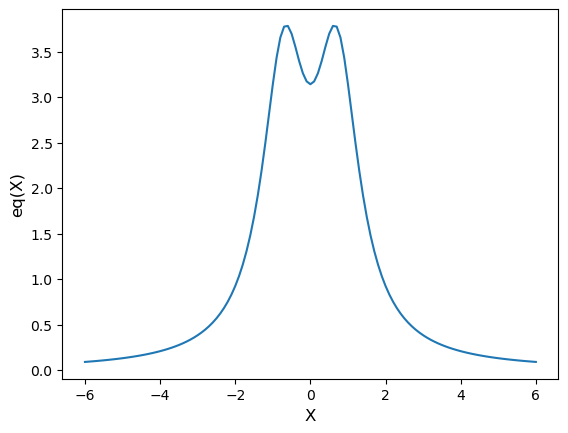
\includegraphics[width=0.75\textwidth]{chapter1-part3-plot3.png}
\end{center}
\end{frame}

%-------------------
% Slide 17: Envelope Rejection Sampling Example
%-------------------
\begin{frame}[fragile]{Envelope Rejection Sampling Example}
\alert{Code}

\vspace{1mm}

\begin{columns}
\column{0.5\textwidth}
{\bf R Code:}
\begin{lstlisting}
n <- 100
counter <- 1
c <- 3.8
target_samples <- vector()

while (counter < n+1) { 
   U <- runif(2)
   proposal <- tan(pi*U[1])
   f <- 1 / (1 + proposal^4)
   g <- 1 / (pi * (1 + proposal^2))
   if (U[2] < f/(c*g)) {
        target_samples[counter] <- proposal
        counter <- counter+1
   }
}
hist(target_samples)
\end{lstlisting}

\column{0.5\textwidth}
{\bf Python Code:}
\begin{lstlisting}
n = 100
c = 3.8
target_samples = []
counter = 0

while counter < n:
    U = np.random.uniform(size=2)
    proposal = np.tan(np.pi * U[0])
    f = 1 / (1 + proposal**4)
    g = 1 / (np.pi * (1 + proposal**2))
    
    if U[1] < f / (c * g):
        target_samples.append(proposal)
        counter += 1

plt.hist(target_samples, bins=20)
plt.show()
\end{lstlisting}
\end{columns}
\end{frame}

%-------------------
% Slide 18: Envelope Rejection Sampling Remarks
%-------------------
\begin{frame}[fragile]{Envelope Rejection Sampling Example}
\begin{center}
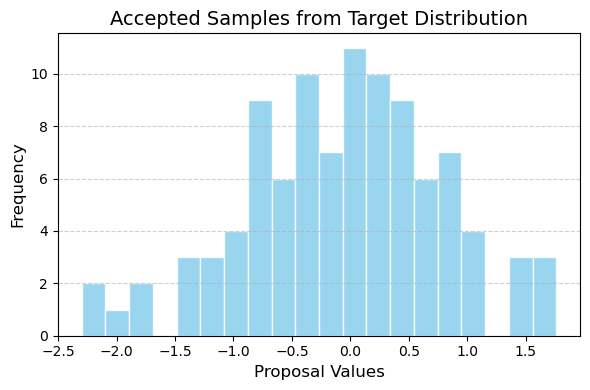
\includegraphics[width=\textwidth]{chapter1-part3-plot4.png}
\end{center}
\end{frame}


%-------------------
% Slide 19: Envelope Rejection Sampling Remarks
%-------------------
\begin{frame}{Envelope Rejection Sampling}
\textbf{Remarks} 

\begin{itemize}
	\item In the code for the previous example, we used the inverse transform method to generate the proposals according to the Cauchy distribution
	\item In this case, we know in advance the sample size for the target distribution. Therefore, we do not know how many ``proposals'' will have to be generated to achieve that. Because of this we use a ``while'' cycle instead of using a ``for'' cycle.
\end{itemize}
\end{frame}

%-------------------
% Slide 20: Homework
%-------------------
\begin{frame}{Homework}
Write a computer program for the implementation of the envelope rejection sampling algorithm to generate a random sample of 1000 random numbers from the distribution given by the density 
\begin{equation*}
f(x)=\left\{ \begin{array}{ll}
\displaystyle{\frac{3x^2+7x^6}{2}} & \text { if } x\in [0,1]\\
0 & \text{otherwise}
\end{array}
\right.
\end{equation*}
Use $U \sim U[0,1]$ as the proposal distribution. On average, how many proposals do we need to generate this random sample? Can you suggest a different choice of proposal distribution so that the algorithm is more efficient (fewer proposals rejected)?
\end{frame}


\end{document}